% !TeX root = Protokoll.tex
% !TeX root = ../../.global/latex/preamble.tex
\subsection{Aufbau}
\begin{figure}[h!]
		\centering
		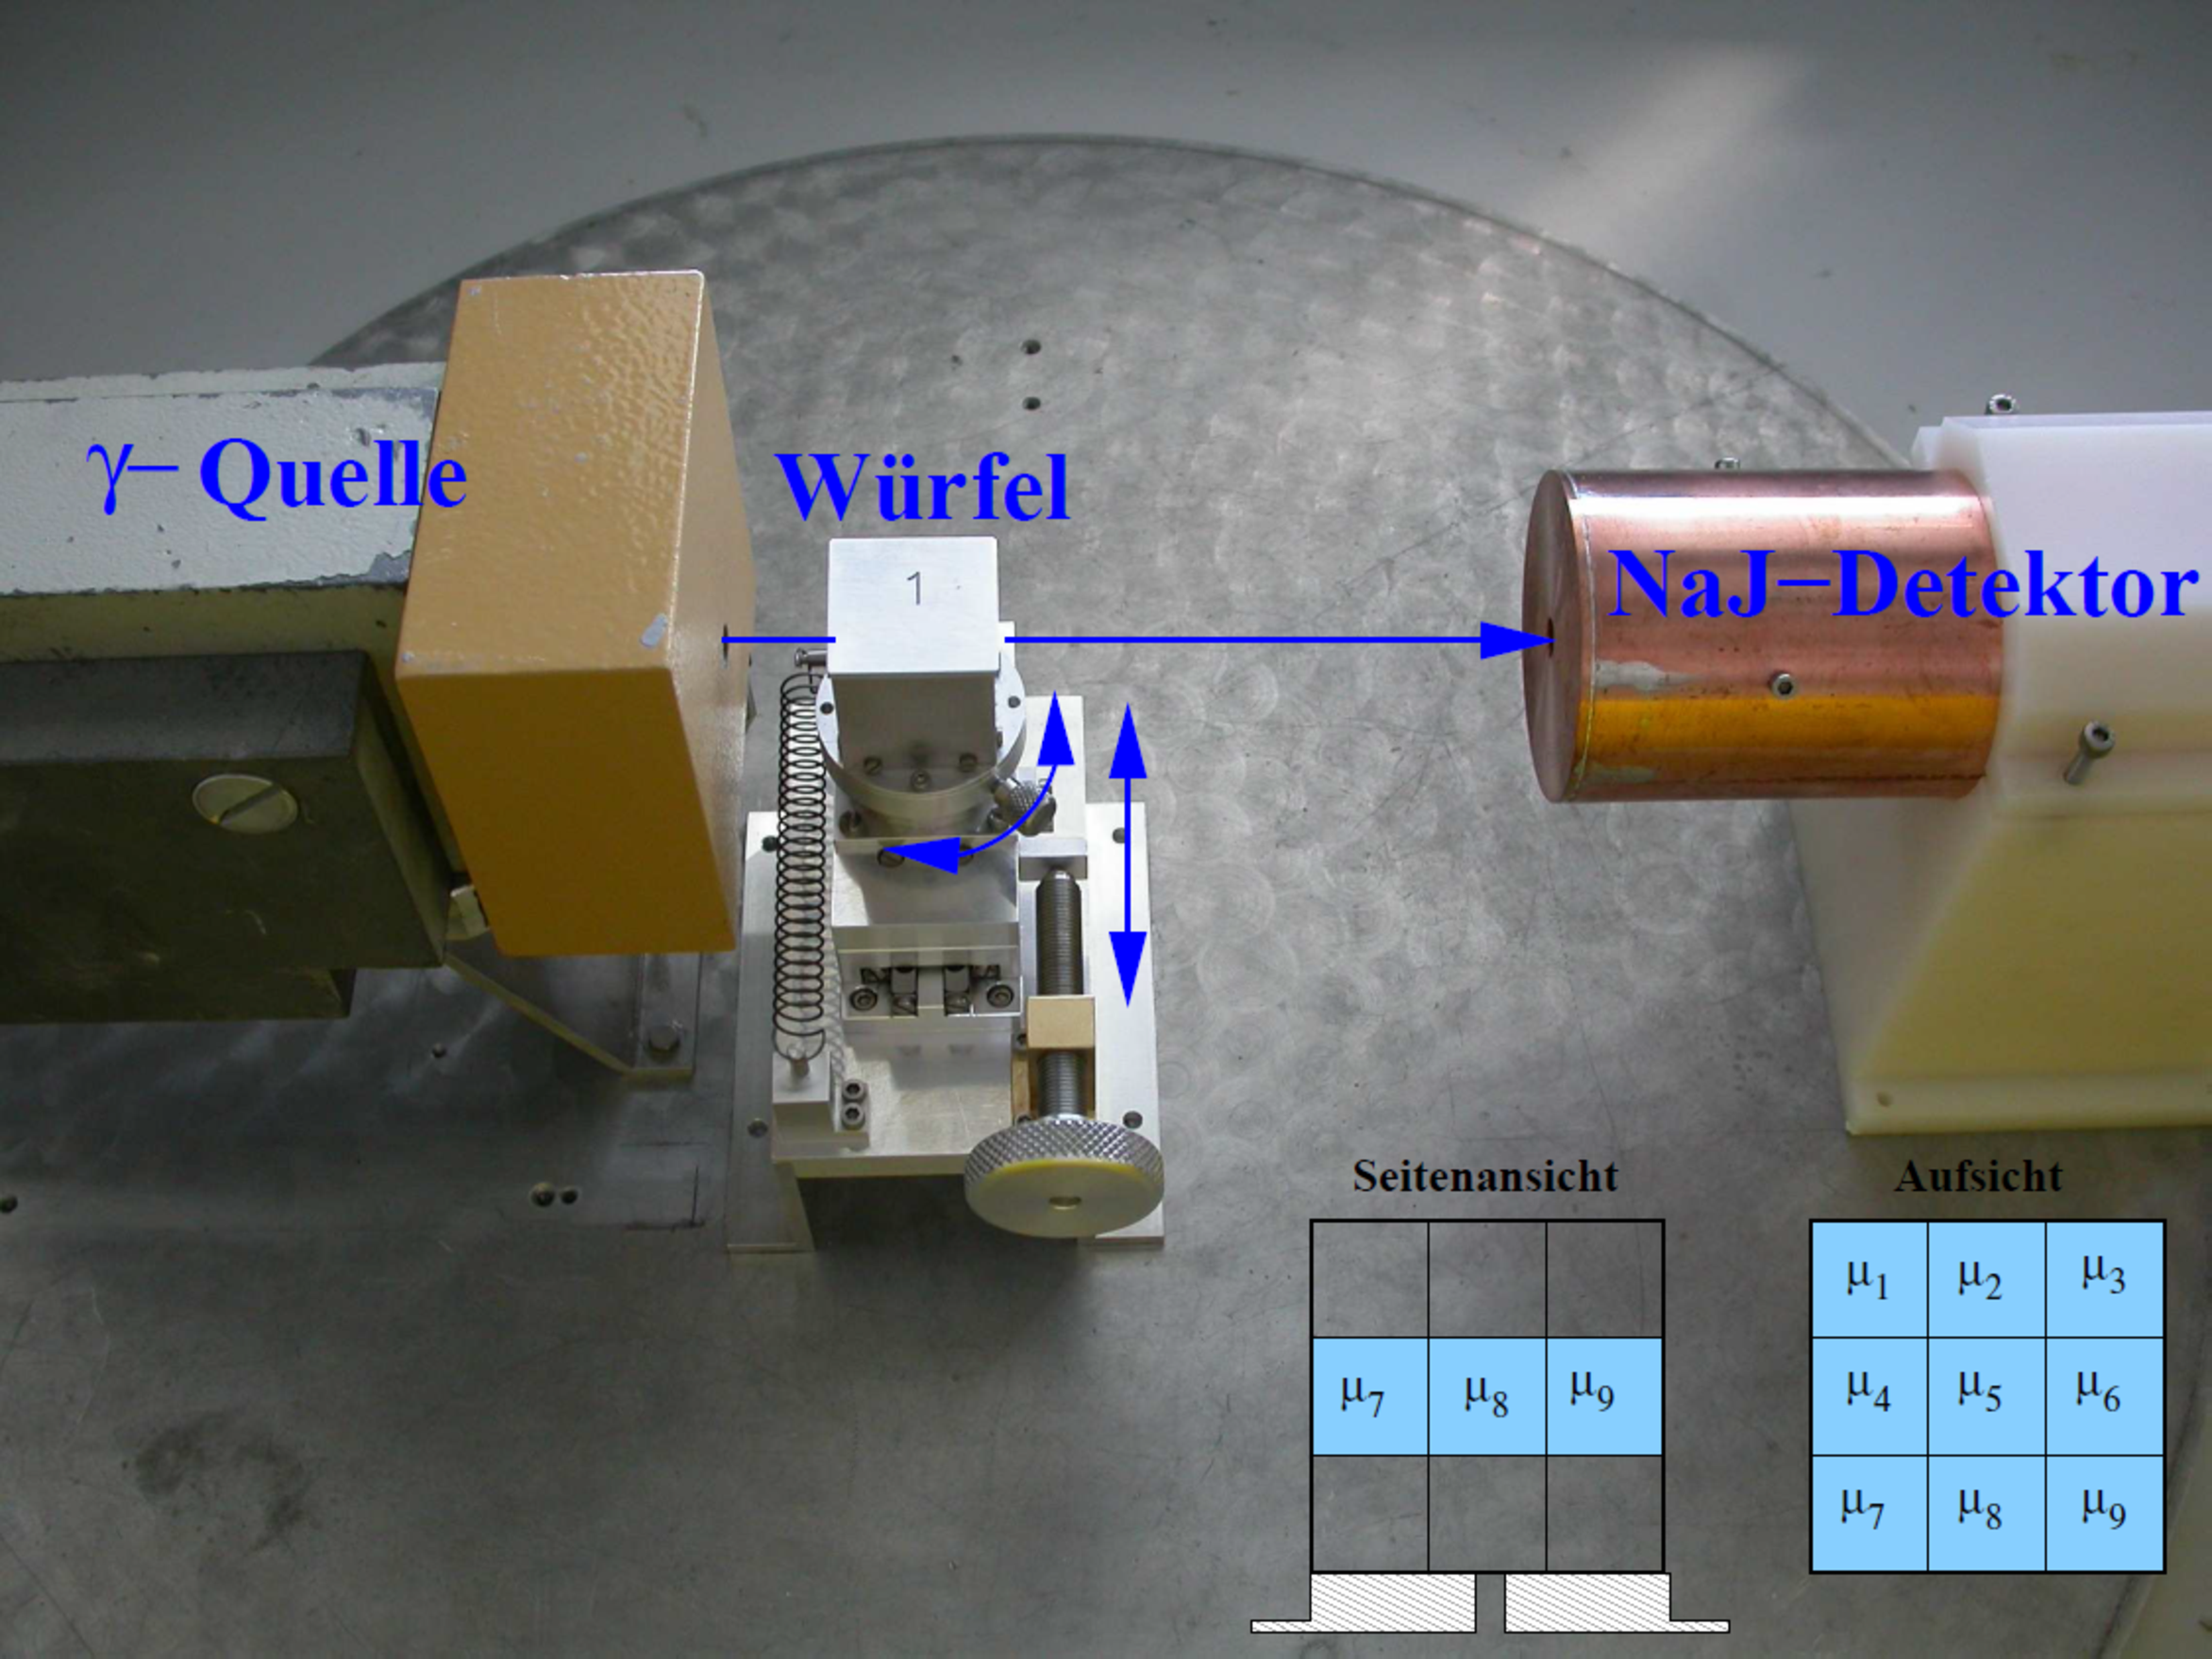
\includegraphics[width = 0.75\textwidth]{../Grafiken/Aufbau.pdf}
		\caption{Hier ist der Versuchsaufbau skizziert. \cite{V27}\label{fig:Versuchsaufbau}}
\end{figure}
\noindent
Der Verwendete Versuchsaufbau ist in \cref{fig:Versuchsaufbau} skizziert.
Die Cd-Lampe wird zwischen Polschuhe eines Elektromagneten gebracht.
Das austretende Licht wird transversal zum Magnetfeld kollimiert und mithilfe eines Glasprismas in seine Farben aufgeteilt und durch einen Spalt kann eine Farbe ab separiert werden.
Durch einen Polarisationsfilter kann die Spektrallinie auf $\pi$- oder $\sigma$-Übergänge untersucht werden.
Unter zu Hilfe nahme einer Lummer-Gehrcke-Platte entsteht ein Interferenzmuster das mit einer Kamera photographiert wird.
Die Lumme-Gehrke-Platte erzeugt mithilfe von Interferenz ein hohes Auflösungsvermögen.
Damit sich zwei Wällenlängen nicht überlagern, darf deren Differenz nicht größer sein als
\begin{align}
	\Delta \lambda_D =\frac{\lambda^2}{2d}\sqrt{\frac{1}{n^2-1}}
\end{align}
sein, dabei ist $d$ die Dicke der Platte und $n$ der Brechungsindes des Matrials für die Wellenlänge.
Das Auflösungsvermögen $A$ das mit so einer Platte erzielt werden kann ist durch
\begin{align}
	A=\frac{\lambda}{\Delta\lambda}=\frac{L}{\Lambda}(n^2-1)
\end{align}
bestimmt, dabei ist $L$ die Länge der Platte.
Die Eigenschaften der verwendeten Lummer-Gehrcke-Platte ist in \cref{tab:Lummer-Gehrcke} aufgeführt.
\begin{table}[h!]
	\centering
	\begin{tabular}{ccccc}
		\toprule
		Farbe & $\lambda/\si{\nano\meter}$& $n$ & $\Delta\lambda_D/\si{\nano\meter}$& $A$\\\midrule
		rot & $\num{643,8}$ & $\num{1,4567}$ & $\num{4.89e-2}$ & $\num{209e3}$\\
		blau & $\num{480,0}$& $\num{1,4635}$ & $\num{2,70e-2}$ & $\num{285e3}$\\\bottomrule
	\end{tabular}
	\caption{Hier sind die Parameter der Lummer-Gehrcke-Platte Aufgeführt, wobei $d=\SI{4}{\milli\meter}$ und $L=\SI{120}{\milli\meter}$ sind. \label{tab:Lummer-Gehrcke}}
\end{table}

\subsection{Messprogramm}
Zunächst wird das Magnetfeld für angelegte Ströme vermessen.
Anschließend wird die Lampe eingeschaltet und die Linsen werden justiert.
Die eigentliche Messung beginnt mit dem $\sigma$-Übergang der roten Linie.
Dazu wird ein Foto der Spektrallinien ohne Magnetfeld gemacht.
Dann wird das Magnetfeld hochgefahren und es wird ein zweites Foto geschossen zu dem Zeitpunkt an dem Sich die Linien soweit aufgeteilt haben, sodass sie unterscheidbar sind, aber noch noch zum Ursprung zurück verfolgt werden können.
Diese Messung wird für die blaue Spektrallinie für die $\pi$- und $\sigma$-Übergänge wiederholt.